\section{Vision}
In order to navigate and insert the Needle at the target it is important to visualise and understand the properties of it for it to communicate with the corresponding kinematic motion.This is done by capturing images of the target on camera.Thus, it is important to know the properties of the camera, how it is transformed from a 2D to a 3D space and how to align them to the appropriate coordinate frames.

\begin{itemize}
    \item Camera Calibration from which we can get the intrinsic and extrinsic properties of the camera
    \item Hand-Eye Calibration which determines the transformation between the robot's end-effector and the camera frame to bind the 3d information of both the coordinate systems
    \item Model Recording, where we get the information such as shape, size, orientation of the experimental object which in our case is the phantom
    \item Model Registration, where we record the images of the phantom as the robot drives the camera around it and stitches the individual point-clouds to a 3d scan and registers with the target model
\end{itemize}

\subsection{Camera Calibration}
This is the first and fundamental step in order to precisely navigate the robot to the target. A camera has two sets of properties- Intrinsic and Extrinsic. The intrinsic properties describe the distortion, focal length and optical centers of the imaging system while the extrinsic properties include the position and orientation of the camera with respect to the world frame. To calibrate and find the parameters, we use the checkerboard with known properties, since it is easier to detect the corners and patterns which is used to estimate the intrinsic parameters. The camera captures the images of checkerboard from different positions and is thus calibrated accordingly.

\subsubsection{Implementation}~\\
To perform camera calibration of a Kinect Camera 2.0, OpenCV2  and python 2.7 were used. The program coded is similar to the classic calibration examples provided in [7]. In order to get a good result with less re-projection error, about 30-40 images were captured and used for the calibration. Higher the number of samples, lesser the error. We were able to validate our results by comparing it with the manufacturer's provided parameters.

Both RGB and depth images were calibrated and from the results we can extract the intrinsic and extrinsic properties of the camera. The extrinsic property gives the transformation from the camera to checkerboard, which is used in hand eye calibration. Kinect2.0 has two cameras one for infrared and depth and one for RGB.
\begin{equation}
cv.stereoCalibrate()
\end{equation}

In order to prevent misalignment between the two cameras, stereo calibration was also performed where we align the depth and RGB cameras which is reflected from the extrinsic results.

\subsection{Eye-in-Hand Calibration}\label{AA}
Hand-Eye calibration is used to determine the transformation between the robot's end-effector and the camera frame. For many robot assisted medical applications, it is necessary to accurately compute the relation between the robot's coordinate system and the coordinate system of a tracking device (camera in our case). We implemented the method from the paper [5] for getting the hand-eye transformation.
\subsubsection{Setup}~\\
We mounted the camera on the end-effector of the robot and we kept the checkerboard stationary as the the calibration object. On moving the robot to different poses, we captured the images as well as the end-effector's position and orientation at each pose which is used in the method explained below. For a precise hand-eye calibration we require at least 35-40 checkerboard poses which should be taken in good light and at different angles. Thus we took all the poses covered inside the hemispherical trajectory.
\subsubsection{Method}~\\
The paper presented a new variation of simultaneously computing both X and Y using a method called QR24 optimisation. The basic equation that is used to solve the hand eye calibration is
\begin{equation}
AX=YB
\end{equation}
\begin{equation}
T_{gripper}^{base} * T_{camera}^{gripper} = T_{marker}^{base} * T_{camera}^{marker}
\end{equation}
From equation (9) we have the transformation from robot's base to gripper(end-effector) as the camera records the checkerboard and the marker poses from the camera to checkerboard. So with two known and two unknown parameters, we can estimate these matrices using a least squares approach and each matrix X and Y will have 12 estimated elements.
\begin{equation}
X = lstsq(A_{combined}, B_{combined})
\end{equation}Thus we get the hand-eye transformation of end-effector to camera using this method.
Working with the simulation model of the Kinect camera gave precise results compared to the ones taken during the experiment since some poses did not give good calibration. But towards the end we managed to take clear photos of the checkerboard and was able to get the transformation which was comparable with the provided result. This result is in turn used while stitching the point-clouds with the target image to get the position of the target.

\subsection{Model Recording}
Model Recording was a short but important phase of the project. This is done to know the the shape, size and the structure of the experimental object which in our case was the phantom.
\subsubsection{Implementation} ~\\
We used the point cloud data of RGB camera which was calibrated. Point cloud is a set of points in space that gives 3D information of the object by placing the points on the external surface. This point-cloud data is usually recorded in the camera coordinate system,but for making the robot to know where the object is exactly placed in the world, the point cloud is to be transferred to world coordinates. Since we got a great resolution and a perfect image on camera, we proceeded with a single point cloud file for model registration.


\subsection{Point-Cloud Stitching and Model Registration}
As the robot drives the camera, with the help of the robot poses and the result from hand-eye calibration.The recorded point clouds are stitched and combined to one point cloud and this is then registered to a high resolution CAD model obtained from computer tomography.Once its registered the target for the needle is selected in the final step.
\begin{figure}[htbp]
\centerline{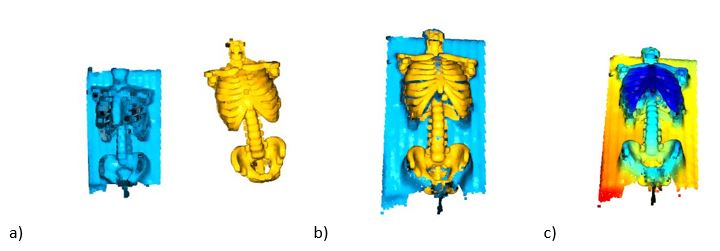
\includegraphics[width =.5\textwidth]{images/finalfig.JPG}}
\caption{a) Initial positions of point-clouds b) Globally registered PointClouds c) Targetpoint selection}
\label{fig}
\end{figure}
\subsubsection{Implementation} ~\\
The phantom was scanned from a single position and we used only one point cloud to perform the registration.
The point-cloud operations were accomplished using Open3D in the version 0.9.0 [6]. It is an open-source library that supports rapid development of software that deals with 3D data.The code was implemented using python 2.7.
The algorithm for performing the model registration and target selection consists of the following steps:
\begin{enumerate}
\item Converting the high resolution CAD model of the phantom to create point-cloud and scale it according to the units used.
\item Stitching and cropping the point cloud so that it only contains the relevant parts
\item Down-sampling the point-clouds and compute Fast Point Feature Histograms(FPFH) features
\item Fast Global Registration using the hand-eye transformation and the obtained pose
\item Local refinement of the registration using point to plane Iterative Closest Point (ICP)
\item Manually choosing the target point from the registered point cloud and transforming it to the world Coordinates.
\end{enumerate}
We used two evaluation metrics, one is the fitness function to measure the overlapping area andthe other is to calculate the RMSE of all inlier correspondences.